\documentclass[10pt,a4paper]{article}
\usepackage[utf8]{inputenc}\usepackage[T1]{fontenc}\usepackage{lmodern}
\usepackage[margin=22mm]{geometry}\usepackage{tikz,booktabs,xurl}
\usetikzlibrary{arrows.meta,positioning}
\usepackage[hidelinks]{hyperref}
\title{HyMeKo: external hypergraph framework survey and matched measurement}
\author{Graph verification infrastructure}\date{Created-at: 2026-10-21 19:49 Europe/Budapest}
\begin{document}\maketitle
\textbf{Scope.} Evaluate HyperNetX 2.4.3, XGI 0.10.2, Hypergraphx 1.8.0 and
Reticula 0.13.0 against the existing canonical-IR workloads. The user's request
authorizes this performance survey. The user selected kato21 and enabled VPN;
SSH with the pinned host key now works. Extend the comparison to graph searches:
source reachability and unit-hyperedge-hop shortest distance from node 0 to the
last declared node. Preserve the native HyMeKo Berge-path/Dijkstra controls.

\textbf{ETA.} One implementation/validation phase, followed by a bounded pilot
and a fresh-process campaign. Package setup and adapter semantics determine the
initial duration; expensive or incompatible cells stop at explicit limits.
Do not promise a full campaign time before the pilot exposes per-call cost.

\textbf{Owner.} Graph owns external benchmark adapters and campaign orchestration.
Core retains canonical IR construction and mathematical generators. Existing
Fixture/IrConstruction exporters supply inputs; external adapters only construct
each library's native object from those exact memberships. The manuscript owns
presentation and receives results only after validation.

\textbf{Discovery.} Existing owners: \texttt{Cell}, \texttt{Evidence},
\texttt{ProcessRunner}, \texttt{Campaign}, \texttt{QuietHostGuard}, the shared
\texttt{pagerank\_support::Fixture}, and the thin canonical-IR gallery exporter.
Extend these entry points; do not duplicate the IR builder, host gate or scheduler.

\begin{center}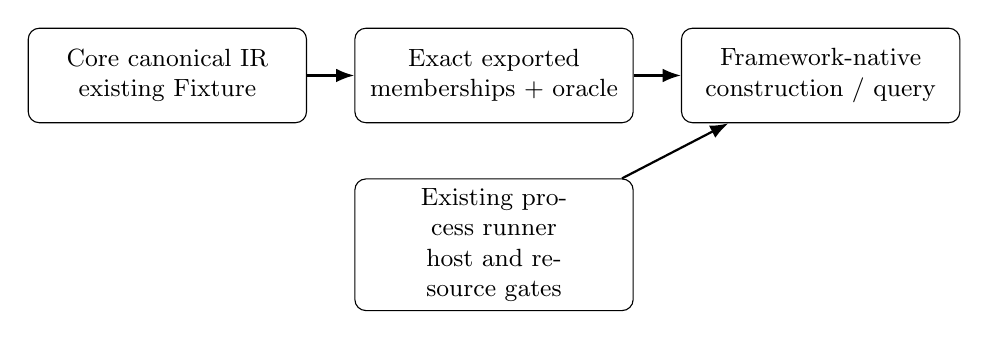
\begin{tikzpicture}[font=\small,box/.style={draw,rounded corners,align=center,text width=33mm,minimum height=12mm},arrow/.style={-{Latex},thick}]
\node[box] (ir) {Core canonical IR\\existing Fixture};
\node[box,right=6mm of ir] (input) {Exact exported\\memberships + oracle};
\node[box,right=6mm of input] (native) {Framework-native\\construction / query};
\node[box,below=7mm of input] (guard) {Existing process runner\\host and resource gates};
\draw[arrow] (ir)--(input);\draw[arrow] (input)--(native);\draw[arrow] (guard)--(native);
\end{tikzpicture}\end{center}


\textbf{Semantic gates.} Components compare complete normalized partitions over
the declared node domain, including isolates. Detect dropped isolated nodes,
duplicate hyperedge collapse and library caches before timing. Cold preparation
and cached queries must have separate labels. PageRank must match the same
vertex--hyperarc--vertex transition, multiplicity, self-return, teleportation,
weights, damping and residual tolerance. A different centrality is not PageRank;
an absent matching API is reported as not matched rather than silently replaced
by our own algorithm under another library's name.
Searches verify the complete reachable set and exact distance against canonical
IR traversal. Label full-source distance APIs versus target queries, scalar
distances versus returned paths, and explicit clique/linegraph projections.

\textbf{Resources and timing.} Fresh subprocesses, explicit opt-in, one algorithm
thread initially, native/BLAS thread counts pinned. Preserve raw timings,
package versions, source/binary/fixture hashes, exceptions and timeouts. Reuse
the existing runner's 180-second process and 16-GiB memory bounds and host gate;
individual operations have a 15-second admission bound. Start small and admit
larger cells only after a successful bounded pilot. Target protocol: five fresh
processes per admitted cell, two warm-ups, nine retained samples; report the
actual batch/repetition scope. Do not compare Windows numbers directly to
retained Linux medians.
The seven prespecified families are chain, hub, eight regions, Steiner triples,
complete 3-uniform, sunflower and Mycielski. Pilot every foreign component,
reachability and shortest-distance call once; retain every successful pilot in
the five-process prepared-query campaign. Preserve all admission failures.
Each fresh process also records its first query as a separate diagnostic of
lazy projection cost; do not pool that single call with warmed samples.

\textbf{Verification.} Inspect installed primary-source APIs. Test isolated and
disconnected nodes, repeated edges, empty inputs and small known partitions.
Where ranking is supported, check the complete vector and an independent
residual. Tests and import checks execute no timed workloads by default.
Only actual current-host native runs qualify as timing evidence.

\textbf{Change surface.} Extend Graph's benchmark-only exporter and
\path{scripts/performance_evidence/} adapters, runner selection, focused tests,
isolated Python dependency lock and phase report. No production Rust algorithm,
public API, Cargo dependency or CORE.YAML edit is planned. No commit, push,
public release or third-party message is authorized by this task.
After validation, update the owning manuscript in
\path{D:/hakiko_ai_ws/01_analysis/zenodo/hymeko_01}: add a bounded external-query
section, import verified CSV/provenance, extend its existing evidence reader and
figure renderer, update the framework table and evidence totals, then rebuild
the PDF and standalone Overleaf ZIP. Its origin was freshly fetched and HEAD
is level with origin/main; existing local manuscript changes are preserved.
Allow about 10--15 minutes after measurement for analysis, layout and packaging.

\textbf{Risks and rollback.} High-arity clique expansion can be quadratic and
exceed memory; cached linegraphs can distort repeated-query timings; isolated
nodes or duplicate edges may disappear during library construction. Fail closed
or label an explicit adapter boundary. Keep the original artifacts and tests.
The Python environment is isolated; removing task-owned adapter changes restores
the old benchmark surface. User and other-agent modifications are preserved.
\end{document}
